% ============================================================
% TRADUÇÃO PT-BR PARA LEITURA — NÃO É A VERSÃO DE SUBMISSÃO.
% A submissão ao ICTAI 2026 é main.tex (inglês). Este arquivo espelha
% main.tex frase a frase, usa o MESMO references_ictai.bib (mesmas chaves
% \cite), as mesmas tabelas/figuras, para conferência lado a lado.
% Qualquer correção de conteúdo deve ser feita primeiro em main.tex e
% depois replicada aqui.
% ============================================================
\documentclass[conference]{IEEEtran}
\IEEEoverridecommandlockouts
\usepackage{cite}
\usepackage{amsmath,amssymb,amsfonts}
\usepackage{graphicx}
\usepackage{booktabs}
\usepackage{multirow}
\usepackage{url}
\usepackage[T1]{fontenc}
\usepackage[utf8]{inputenc}
\usepackage[english,brazil]{babel}

\begin{document}

\title{Ulysses-MTRAG: Um Benchmark Sintético Multi-Turno para\\
Geração Aumentada por Recuperação sobre Texto Legal Brasileiro}

\author{\IEEEauthorblockN{[Cópia de leitura em português --- ver main.tex para a submissão]}
\IEEEauthorblockA{\textit{Tradução não-oficial, apenas para revisão interna}\\
anonymous@example.org}}

\maketitle

\begin{abstract}
A geração aumentada por recuperação (RAG) para assistência jurídica é
inerentemente conversacional; no entanto, os recursos existentes de recuperação
de informação jurídica em português brasileiro são de turno único e param na
recuperação. Apresentamos o \textbf{Ulysses-MTRAG}, um benchmark sintético de RAG
multi-turno para o diálogo legislativo brasileiro. Cada sessão ancora seu
primeiro turno em uma consulta real de especialista que carrega julgamentos
humanos de relevância (Ulysses-RFCorpus); um LLM então gera turnos de
continuação coerentes, e um juiz LLM distinto do gerador avalia a relevância dos
documentos recuperados. Usando o benchmark, respondemos a três perguntas.
Primeira: como a qualidade da recuperação evolui ao longo dos turnos, e o
histórico do diálogo ajuda? Sob quatro estratégias de contexto e dois
recuperadores, a qualidade degrada significativamente com a profundidade do
turno, e a melhor estratégia é \emph{dependente do recuperador}: a recuperação
densa não melhora com o histórico em relação ao turno corrente sozinho, enquanto
o BM25 lexical é significativamente melhor com o histórico completo do diálogo,
que atua como expansão de consulta. Segunda: a escala do modelo melhora a
fidelidade da geração? Um estudo controlado por tamanho e família (de 7B a 72B
parâmetros) mostra que a família do modelo domina a contagem de parâmetros: um
bom modelo de 8B é mais fiel que modelos de 14B e 31B de outras famílias e
competitivo com um modelo de 72B nove vezes maior, enquanto a degradação da
recuperação se propaga para a geração apenas fracamente (Spearman
$\rho\!\le\!0.21$). Terceira: quão confiável é o juiz LLM de relevância? Frente
aos rótulos de especialistas pré-existentes, a concordância no pool completo é
modesta ($0.58$)---dominada por documentos do pool que os especialistas nunca
avaliaram---mas sobe para $0.94$ no subconjunto que eles rotularam
explicitamente. Disponibilizaremos o benchmark, os prompts e o código; um
repositório anonimizado acompanha esta submissão.
\end{abstract}

\begin{IEEEkeywords}
geração aumentada por recuperação, diálogo multi-turno, PLN jurídico,
recuperação de informação, LLM-como-juiz, português brasileiro
\end{IEEEkeywords}

% ============================================================
\section{Introdução}
A busca por informação jurídica é conversacional: um analista refina uma
pergunta inicial ao longo de vários turnos. A geração aumentada por recuperação
(RAG) \cite{Lewis2020RAG} é o paradigma dominante para fundamentar esse tipo de
assistência, mas os recursos de RI jurídica em português brasileiro---o
Ulysses-RFCorpus \cite{Vitorio2024}, o JurisTCU \cite{Fernandes2026JurisTCU} e o
benchmark JU\'A \cite{Pereira2026JUA}---são de \emph{turno único} e param na
recuperação. O RAG jurídico multi-turno em português, até onde sabemos, ainda
não foi estudado.

Atacamos essa lacuna com o \textbf{Ulysses-MTRAG}, um benchmark sintético
multi-turno para o diálogo legislativo brasileiro. Em vez de transplantar uma
receita existente, nossa construção mira tanto escalabilidade quanto validade
ecológica: cada sessão é ancorada em uma consulta \emph{real} de especialista que
carrega julgamentos humanos de relevância, e apenas os turnos de continuação são
gerados por LLM. Esse desenho ancorado em humanos distingue o Ulysses-MTRAG dos
benchmarks multi-turno anteriores. O MTRAG \cite{Katsis2025MTRAG} é inteiramente
escrito por humanos---preciso, porém não escalável. O CORAL
\cite{Cheng2025CORAL} deriva conversas automaticamente da Wikipédia---escalável,
porém sem \emph{ground truth} de relevância de especialistas. Ancorar em
julgamentos de especialistas pré-existentes nos permite fazer algo que nenhum
dos dois desenhos anteriores viabiliza: auditar o juiz LLM de relevância contra
especialistas \emph{dentro} do próprio benchmark. Nossas contribuições são:
\begin{itemize}
  \item \textbf{Ulysses-MTRAG}: um benchmark de RAG jurídico multi-turno com 100
  sessões de quatro turnos sobre 105{,}669 projetos de lei, com primeiros turnos
  ancorados em humanos, continuações geradas por LLM e rótulos de relevância em
  pool atribuídos por um juiz distinto do gerador.
  \item Uma \textbf{análise de recuperação multi-turno} sobre quatro estratégias
  de contexto e dois recuperadores, com testes pareados de significância,
  mostrando degradação por turno e uma interação estratégia--recuperador: o uso
  ótimo do histórico do diálogo se inverte entre a recuperação densa e a
  lexical.
  \item Um \textbf{estudo de geração controlado por tamanho e família}
  (7B--72B) mostrando que o melhor modelo de 8B supera modelos de 14B e 31B de
  outras famílias e é estatisticamente indistinguível de um modelo de 72B nove
  vezes maior. Aumentar a escala não é, portanto, um caminho confiável para RAG
  jurídico fiel neste domínio.
  \item Evidência de que \textbf{a degradação da recuperação se propaga para a
  geração apenas fracamente}: a fidelidade declina de forma bem menos acentuada
  que a qualidade da recuperação ao longo dos turnos, e se correlaciona
  fracamente com ela no nível do turno.
  \item Uma \textbf{avaliação de confiabilidade} do juiz LLM de relevância
  contra rótulos de especialistas pré-existentes, desemaranhando o fator de
  confusão da incompletude do pooling: no subconjunto de documentos que os
  especialistas rotularam explicitamente, a concordância bruta é $0.94$.
\end{itemize}

\noindent\textbf{Questões de pesquisa.}
\textbf{RQ1}: Como a qualidade da recuperação evolui ao longo dos turnos, e
estratégias de contexto cientes do histórico superam o uso apenas da consulta
corrente? \textbf{RQ2}: Quão confiável é o juiz LLM de relevância frente aos
rótulos de especialistas? \textbf{RQ3}: A escala do modelo melhora a geração
fundamentada em diálogo, e a degradação da recuperação se propaga para as
respostas geradas?

% ============================================================
\section{Trabalhos Relacionados}
\textbf{Avaliação de RAG e LLM-como-juiz.} Juízes LLM são hoje padrão para
avaliar geração \cite{Zheng2023MTBench,Liu2023GEval,Kim2024Prometheus2} e RAG
especificamente \cite{Es2024RAGAS}, incluindo a avaliação de relevância
\cite{Thomas2024Searcher,Upadhyay2024UMBRELA,Faggioli2023Perspectives}. Eles
carregam vieses conhecidos---posição \cite{Wang2024Unfair}, verbosidade
\cite{Zheng2023MTBench} e autopreferência \cite{Panickssery2024SelfPref}---o que
motiva nosso uso de um juiz distinto do gerador. Rótulos de relevância também
são altamente sensíveis ao prompt \cite{Arabzadeh2025Prompt}; em vez de um rigor
cego, adotamos uma rubrica com \emph{reason-then-label} \cite{Liu2023GEval} e
quantificamos a concordância com rótulos de especialistas, reportando
estatísticas de concordância \cite{Calderon2025AltTest,Hashemi2024LLMRubric}.

\textbf{RAG multi-turno / conversacional.} Benchmarks de QA e RAG
conversacionais \cite{Katsis2025MTRAG,Cheng2025CORAL,Qu2020ORConvQA} e reescrita
conversacional de consultas \cite{Anantha2021QReCC,Elgohary2019CANARD,Mao2023LLM4CS}
estabelecem as estratégias de contexto que comparamos. Se o histórico ajuda é
uma questão em aberto: o ORConvQA \cite{Qu2020ORConvQA} encontra benefício do
histórico em dados humanos, enquanto pipelines sintéticos tendem a produzir
perguntas autossuficientes \cite{Vlachos2025Synthetic}---descontextualizadas no
sentido de \cite{Choi2021Decontextualization}---uma tendência que nosso
benchmark permite quantificar e testar sob estresse. A degradação em diálogos
longos também está documentada \cite{Laban2025Lost}. Em relação ao MTRAG e ao
CORAL, o Ulysses-MTRAG difere em três eixos: proveniência dos turnos (semente
humana + continuações sintéticas, vs.\ totalmente humano no MTRAG e totalmente
automático no CORAL), proveniência dos rótulos de relevância (julgamentos de
especialistas no turno-semente, viabilizando a auditoria do juiz dentro do
benchmark), e domínio (projetos de lei em português, incluindo um cenário de
língua de poucos recursos que nenhum dos dois cobre).

\textbf{Recuperação de documentos longos e chunking.} A indexação em nível de
passagem de documentos longos é a mitigação canônica quando as entradas excedem
os limites dos modelos \cite{Dai2019Deeper,Karpukhin2020DPR}, embora a
granularidade ótima da unidade de recuperação siga em debate
\cite{Jiang2024LongRAG}. Modelos de embedding têm limites rígidos de tokens
(BGE-M3: 8192 tokens \cite{Chen2024BGEM3}) e degradam em entradas longas
\cite{Zhou2024LengthCollapse}; o BM25 permanece uma baseline forte,
especialmente em domínios lexicalmente ricos \cite{Robertson2009BM25,Thakur2021BEIR}.

\textbf{RI jurídica em português e dados sintéticos.} Construímos sobre os
recursos brasileiros de RI jurídica
\cite{Vitorio2024,Fernandes2026JurisTCU,Pereira2026JUA,Junior2025BRTaxQA,LuzdeAraujo2018LeNERBr}.
A geração de dados sintéticos com LLMs está bem estabelecida para RI
\cite{Bonifacio2022InPars,Dai2023Promptagator} e como proxy de avaliação
\cite{Chiang2023Can}; ancorar dados sintéticos em \emph{ground truth} humano
mitiga os riscos da geração totalmente recursiva \cite{Shumailov2024Collapse}.

% ============================================================
\section{Configuração de Recuperação}
\label{sec:foundation}
Nossos experimentos usam dois recuperadores padrão: o lexical BM25
\cite{Robertson2009BM25} e o denso BGE-M3 \cite{Chen2024BGEM3}. O corpus do
benchmark é composto por projetos de lei, cujos resumos oficiais
(\emph{ementas}) são curtos e cabem confortavelmente na janela do codificador.
Os experimentos multi-turno, portanto, indexam cada projeto pelo resumo
inteiro, sem necessidade de chunking.

\textbf{Uma fronteira de comprimento, e por que nosso benchmark a evita.} Antes
da análise multi-turno, verificamos se essa pilha de recuperação tem uma
limitação de comprimento em texto legal brasileiro, usando o subdomínio
regulatório do JU\'A \cite{Pereira2026JUA} (NormasTCU; normas de
$\sim$12 mil tokens, $n{=}46$ consultas) como teste de estresse. E tem: ali, a
recuperação densa de documento inteiro \emph{colapsa}---nenhuma norma relevante
aparece em nenhum top-10, resultando em nDCG@10$=$0.000 em todas as
consultas---enquanto o BM25 lexical atinge 0.328 (Tabela~\ref{tab:chunking}). O
mecanismo é o comprimento: cada norma excede em muito a janela de 8192 tokens do
BGE-M3, de modo que o vetor único indexado por documento é calculado a partir de
um prefixo truncado que omite as passagens relevantes à consulta
\cite{Chen2024BGEM3,Zhou2024LengthCollapse}. O remédio padrão em nível de
passagem---dividir cada norma em blocos de menos de 8 mil tokens, indexar os
blocos e mapear os blocos recuperados de volta aos documentos
\cite{Dai2019Deeper,Karpukhin2020DPR}---recupera a recuperação densa até a
paridade com o BM25 (nDCG@10$=$0.330; o BM25 ainda mantém recall melhor). Isso
confirma que a fronteira é real e nos dá uma mitigação testada, mas o nosso
próprio corpus de projetos de lei nunca se aproxima dela: os resumos dos
projetos ficam bem abaixo de 8 mil tokens, então o benchmark multi-turno abaixo
os indexa por inteiro, sem necessidade de chunking.

\begin{table}[t]
\caption{Recuperação no NormasTCU ($n{=}46$). A recuperação densa de documento
inteiro colapsa em normas de $\sim$12 mil tokens; a indexação por blocos
recupera a paridade com o BM25.}
\label{tab:chunking}
\centering
\begin{tabular}{lcccc}
\toprule
\textbf{Método} & \textbf{nDCG@5} & \textbf{nDCG@10} & \textbf{R@10} & \textbf{MRR} \\
\midrule
BM25 (texto completo)     & 0.287 & \textbf{0.328} & 0.339 & 0.454 \\
Denso, documento inteiro  & 0.000 & 0.000 & 0.000 & 0.000 \\
Denso, nível de bloco     & 0.317 & \textbf{0.330} & 0.294 & 0.559 \\
\bottomrule
\end{tabular}
\end{table}

% ============================================================
\section{O Benchmark Ulysses-MTRAG}
\label{sec:benchmark}
\textbf{Construção.} A construção das sessões tem três etapas: seleção de
sementes, geração de turnos e controle de qualidade.

\emph{Seleção de sementes.} Partimos das 692 consultas da versão pública do
Ulysses-RFCorpus, cada uma carregando julgamentos graduados de relevância
(relevante / parcialmente relevante / irrelevante) produzidos pelos consultores
legislativos da Câmara dos Deputados \cite{Vitorio2024}, sobre um corpus de
105{,}669 projetos de lei.\footnote{As contagens referem-se à versão pública que
usamos (692 consultas; 105{,}669 projetos); o artigo do dataset reporta 693
consultas e 105{,}681 documentos \cite{Vitorio2024}.} Mantemos apenas as
consultas com pelo menos três projetos (parcialmente) relevantes, embutimos os
textos das consultas restantes com BGE-M3 e as agrupamos com $k$-means
($k{=}100$, semente fixa). Uma consulta representativa por cluster vira uma
semente de sessão, resultando em um conjunto diverso e não redundante de 100
sementes; cada semente vira o Turno~1 e herda seus rótulos de relevância de
especialistas.

\emph{Geração de turnos.} Os Turnos~2--4 são gerados por um LLM instruído
(Qwen2.5-72B), condicionado ao histórico completo da sessão e instruído a
produzir uma próxima pergunta coerente de um tipo \emph{prescrito}---continuação
(\emph{follow-up}), esclarecimento, não autossuficiente
(\emph{non-standalone}), comparativa ou temporal. Desenhamos esse esquema de
cinco tipos em torno dos desafios conversacionais que o MTRAG enfatiza:
perguntas não autossuficientes e comparativas, e respondibilidade
\cite{Katsis2025MTRAG}.

\emph{Controle de qualidade.} O gerador é instruído a manter o tópico e não
repetir turnos anteriores. Descartamos gerações degeneradas---vazias,
duplicadas ou fora de tópico---e as regeneramos. O resultado são 100 sessões de
quatro turnos (400 turnos no total); a Fig.~\ref{fig:example} mostra uma delas.
Um gerador especializado em português (p.ex., Gaia/Sabi\'a) fica como trabalho
futuro.

\begin{table}[t]
\caption{Composição do Ulysses-MTRAG: distribuições realizadas de tipo de turno
e tipo de resposta sobre os 300 turnos gerados (T2--T4). Os tipos de turno são
prescritos por amostragem no momento da geração; os tipos de resposta são os
rotulados pelo gerador.}
\label{tab:stats}
\centering
\begin{tabular}{lr@{\hspace{1.2em}}lr}
\toprule
\textbf{Tipo de turno} & \textbf{\%} & \textbf{Tipo de resposta} & \textbf{\%} \\
\midrule
continuação          & 47.0 & respondível     & 99.3 \\
esclarecimento       & 20.3 & parcial         &  0.7 \\
não autossuficiente  & 11.3 & não respondível &  0.0 \\
comparativa          & 11.0 &                 &      \\
temporal             & 10.3 &                 &      \\
\bottomrule
\end{tabular}
\end{table}

A Tabela~\ref{tab:stats} reporta a composição realizada. Como a distribuição de
tipos é um insumo da construção (amostrada por desenho), não a lemos como um
achado; o que \emph{é} informativo é que apenas $11.3\%$ dos turnos gerados são
explicitamente não autossuficientes, de modo que o benchmark---como outros
pipelines sintéticos de QA conversacional \cite{Vlachos2025Synthetic}---consiste
majoritariamente de perguntas autossuficientes (descontextualizadas
\cite{Choi2021Decontextualization}) sobre um tópico compartilhado. Tratamos
isso como uma propriedade mensurável da receita de construção sintética e
testamos suas consequências sob estresse na Seção~\ref{sec:results} (RQ1),
incluindo uma análise estratificada por tipo de turno. Quase todos os turnos são
respondíveis ($99.3\%$); a quase ausência de turnos não respondíveis é uma
limitação que discutimos na Seção~\ref{sec:discussion}.

\textbf{Rótulos de relevância.} Para cada turno, os documentos recuperados por
todas as estratégias de contexto são reunidos em um pool e rotulados uma única
vez por um juiz LLM (Llama-3.3-70B), \emph{distinto do gerador} para evitar
viés de autopreferência \cite{Panickssery2024SelfPref}, usando uma rubrica
graduada com \emph{reason-then-label} \cite{Liu2023GEval}. \emph{Todos} os
escores de recuperação deste artigo, incluindo o Turno~1, usam esses rótulos do
juiz, de modo que as comparações entre turnos repousam sobre uma única fonte de
rótulos; os rótulos de especialistas do Turno~1 são reservados para auditar o
próprio juiz (Seção~\ref{sec:results}, RQ2). Rótulos graduados são binarizados
em $0.5$ (parcialmente relevante conta como relevante) sempre que a
concordância binária é computada.

\begin{figure}[t]
\small\setlength{\parindent}{0pt}
\textbf{T1} \emph{(semente, rótulo humano)}: ``Criação de fundo para prevenção de desastres naturais e e recuperação de seus efeitos, para\ldots''\\
$\rightarrow$ top: \textbf{PL 295/2007} --- \emph{relevante}\\[3pt]
\textbf{T2} \emph{(continuação)}: ``Quais são os principais critérios e mecanismos de distribuição dos recursos do fundo para\ldots''\\
$\rightarrow$ top: \textbf{PL 5067/2016} --- \emph{relevante}\\[3pt]
\textbf{T3} \emph{(esclarecimento)}: ``Em quais situações específicas os recursos do fundo para prevenção de desastres naturais e\ldots''\\
$\rightarrow$ top: \textbf{PL 10898/2018} --- \emph{relevante}\\[3pt]
\textbf{T4} \emph{(esclarecimento)}: ``Como são definidas as prioridades para a alocação de recursos do fundo em situações de\ldots''\\
$\rightarrow$ top: \textbf{PL 4450/2020} --- \emph{parcialmente relevante}
\caption{Um exemplo trabalhado do Ulysses-MTRAG: uma sessão de quatro turnos
semeada por uma consulta real do Ulysses-RFCorpus (T1, que adicionalmente
carrega rótulos de especialistas), com continuações geradas por LLM (T2--T4).
Para cada turno mostramos o projeto de lei mais bem recuperado e seu rótulo de
relevância do juiz LLM. As consultas são reproduzidas verbatim no português
original, incluindo erros de digitação presentes no corpus-fonte. O projeto
recuperado \emph{muda} ao longo dos turnos e degrada para apenas
\emph{parcialmente relevante} no T4.}
\label{fig:example}
\end{figure}

% ============================================================
\section{Configuração da Avaliação Multi-Turno}
\label{sec:setup}
\textbf{Recuperação.} Para cada turno recuperamos os top-$k$ ($k{=}10$)
projetos sob quatro estratégias de contexto: \emph{last-turn} (apenas a
consulta corrente), \emph{concat} (consultas anteriores pré-anexadas),
\emph{full-history} (todos os turnos anteriores) e \emph{rewrite} (um modelo
Llama-3.1-8B reescreve a consulta para a forma autossuficiente)
\cite{Mao2023LLM4CS,Elgohary2019CANARD}. Por turno e por recuperador, reunimos
em pool os documentos recuperados pelas quatro estratégias e julgamos o pool
uma única vez (pooling padrão), pontuando cada estratégia com nDCG@10 sobre os
rótulos compartilhados. Um cache persistente de julgamentos atribui rótulos
idênticos a qualquer par (consulta, documento) que apareça nos pools de ambos
os recuperadores. Rodamos a comparação completa de estratégias sob \emph{ambos}
os recuperadores---denso BGE-M3 e lexical BM25 (\S\ref{sec:foundation})---para
testar se as conclusões sobre o histórico do diálogo são específicas do
recuperador.

\textbf{Geração.} Para testar se a degradação da recuperação se propaga para as
respostas, os top-5 projetos recuperados via last-turn de cada turno são
passados, com um prompt ciente do histórico, a cinco modelos de linguagem
pequenos (SLMs) de pesos abertos e instruídos. Escolhemos esses cinco para
cobrir a faixa de tamanhos com qualidade competitiva: Qwen2.5-7B
\cite{Qwen2024Qwen25}, Qwen3-8B \cite{Yang2025Qwen3}, Ministral-8B, Phi-4 (14B)
\cite{Abdin2024Phi4}, e Gemma-4-31B. Esse espalhamento permite que o efeito da
escala seja lido diretamente da comparação. Pontuamos cada resposta em três
eixos adaptados da avaliação de geração do MTRAG \cite{Katsis2025MTRAG}:
(i) \emph{fidelidade ao contexto} (sem referência, estilo RAGAS
\cite{Es2024RAGAS}), julgada pelo Llama-3.3-70B \cite{Grattafiori2024Llama3};
(ii) \emph{similaridade à referência} a uma resposta-oráculo via BERTScore-F1
\cite{Zhang2020BERTScore} e ROUGE-L \cite{Lin2004ROUGE}; e (iii) uma comparação
por juiz LLM contra a resposta do oráculo. O oráculo (Qwen2.5-72B) recebe o
\emph{mesmo} contexto recuperado e histórico que os modelos avaliados. Dois
fatos de desenho precisam ser ditos abertamente: o oráculo é o mesmo modelo que
gerou as perguntas de continuação, e ele compartilha família com dois modelos
avaliados. O juiz é distinto tanto dos geradores quanto do oráculo, e nossas
afirmações principais repousam sobre o eixo de fidelidade sem referência, que
não usa o oráculo; empiricamente, as métricas baseadas em referência tampouco
favorecem a família do oráculo (o Phi-4 lidera ambas, \S\ref{sec:results}).

\textbf{Implementação.} A geração usa temperatura $0.1$ (máx.\ 1024 tokens); o
julgamento usa temperatura $0$. A recuperação densa usa embeddings BGE-M3 com
FAISS \cite{Douze2024Faiss}; o BM25 é o BM25Okapi ($k_1{=}1.5$, $b{=}0.75$); o
chunking do NormasTCU usa blocos de 3{,}000 caracteres com sobreposição de 400;
o agrupamento de sementes usa $k$-means com semente aleatória fixa. O BERTScore
usa BERT multilíngue. Os modelos são acessados por APIs compatíveis com OpenAI.
Todos os prompts (geração de turnos, reescrita de consultas, rubrica de
relevância, julgamento de fidelidade), identificadores de modelos e arquivos de
configuração estão incluídos no repositório anonimizado que acompanha esta
submissão.

% ============================================================
\section{Resultados}
\label{sec:results}
\textbf{RQ1 --- degradação por turno e a interação estratégia--recuperador.}
A Tabela~\ref{tab:mtrag} reporta o nDCG@10 por recuperador, estratégia e turno;
as estratégias coincidem no T1, onde não existe histórico. Sob ambos os
recuperadores, a qualidade da recuperação \emph{declina significativamente
conforme a conversa se aprofunda}: para o last-turn denso, o nDCG@10 cai de
$0.876$ (semente) para $0.617$ no T3 ($\Delta{=}0.26$, Wilcoxon pareado
$p<10^{-12}$; Fig.~\ref{fig:retrieval}). A maior queda isolada (T1$\to$T2)
coincide com a troca de consultas-semente escritas por humanos para
continuações sintéticas, de modo que lemos a degradação com a profundidade
primariamente no declínio contínuo dentro dos turnos sintéticos.

\emph{Qual estratégia de contexto é melhor depende do recuperador.} Para o
denso BGE-M3, nenhuma estratégia ciente do histórico supera o last-turn (médias
dentro de $\approx$0.02; last-turn é indistinguível de concat e full-history,
Holm $p\ge0.17$, e melhor que rewrite, $p_{\text{adj}}{=}0.023$): concatenar o
histórico dilui o embedding único da consulta. Para o BM25 lexical o ranking
\emph{se inverte}---full-history é a melhor e last-turn a \emph{pior} estratégia
($0.741$ vs.\ $0.668$ de média geral; diferença de $+0.097$ em T2--T4, Wilcoxon
pareado $p<10^{-7}$)---porque anexar os turnos anteriores atua como expansão de
consulta, fornecendo termos jurídicos lexicalmente correspondentes. Usar apenas
o turno corrente é, portanto, um padrão seguro para a recuperação densa, mas
uma escolha ruim para a recuperação lexical, onde vale o oposto. Essa interação
alerta contra tirar conclusões sobre contexto conversacional a partir de um
único recuperador.

Estratificar os resultados densos por tipo de turno localiza o resultado nulo
do last-turn: turnos explicitamente não autossuficientes são os mais difíceis
(last-turn nDCG@10 $0.52$ vs.\ $0.64$--$0.73$ para os demais tipos) e as
estratégias densas cientes do histórico não os recuperam (concat $0.40$,
full-history $0.43$, rewrite $0.40$), enquanto o full-history ajuda apenas
modestamente em turnos de esclarecimento ($0.69$ vs.\ $0.66$) e temporais
($0.68$ vs.\ $0.64$)---consistente com as perguntas autossuficientes que
pipelines sintéticos sabidamente produzem \cite{Vlachos2025Synthetic},
descontextualizadas no sentido de \cite{Choi2021Decontextualization}; em
contraste com o ORConvQA \cite{Qu2020ORConvQA}, onde o histórico ajuda em
diálogo humano. Uma ressalva: os documentos do pool são julgados contra o texto
do próprio turno, o que pode favorecer o last-turn justamente nos turnos não
autossuficientes; julgamento ciente do histórico é trabalho futuro.

\begin{table}[t]
\caption{Recuperação multi-turno (nDCG@10) por recuperador, estratégia de
contexto e posição do turno (100 conversas; por recuperador, um único pool
julgado por LLM pontua todas as estratégias por turno, incluindo o T1---por
isso as estratégias coincidem no T1). Melhor estratégia por recuperador (média
geral) em negrito. A ordenação \emph{se inverte} entre recuperação densa e
lexical.}
\label{tab:mtrag}
\centering\small\setlength{\tabcolsep}{4pt}
\begin{tabular}{llccccc}
\toprule
\textbf{Recup.} & \textbf{Estratégia} & \textbf{T1} & \textbf{T2} & \textbf{T3} & \textbf{T4} & \textbf{média} \\
\midrule
\multirow{4}{*}{\rotatebox[origin=c]{90}{BGE-M3}}
 & last-turn    & 0.876 & 0.727 & 0.617 & 0.636 & \textbf{0.714} \\
 & rewrite      & 0.876 & 0.718 & 0.587 & 0.604 & 0.696 \\
 & concat       & 0.876 & 0.718 & 0.621 & 0.557 & 0.693 \\
 & full-history & 0.876 & 0.695 & 0.605 & 0.597 & 0.693 \\
\midrule
\multirow{4}{*}{\rotatebox[origin=c]{90}{BM25}}
 & full-history & 0.900 & 0.755 & 0.670 & 0.637 & \textbf{0.741} \\
 & concat       & 0.900 & 0.731 & 0.624 & 0.449 & 0.676 \\
 & rewrite      & 0.900 & 0.652 & 0.587 & 0.564 & 0.676 \\
 & last-turn    & 0.900 & 0.641 & 0.580 & 0.551 & 0.668 \\
\bottomrule
\end{tabular}
\end{table}

\begin{figure}[t]
\centering
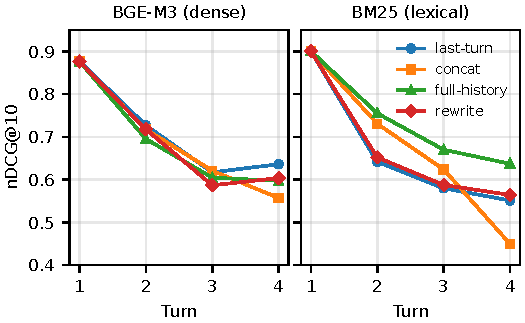
\includegraphics[width=\columnwidth]{fig_retrieval_turns.pdf}
\caption{nDCG@10 de recuperação por turno para as quatro estratégias de
contexto, sob recuperação densa (esquerda) e lexical (direita) (100 conversas).
A qualidade cai após o turno-semente em ambos, mas a melhor estratégia
\emph{se inverte}: last-turn lidera nos embeddings densos, full-history lidera
no BM25.}
\label{fig:retrieval}
\end{figure}

\textbf{RQ2 --- confiabilidade do juiz frente aos rótulos de especialistas.}
Auditamos o juiz LLM contra os rótulos de especialistas pré-existentes no pool
do Turno~1 da execução densa, reportando a concordância bruta junto do
$\kappa$ de Cohen \cite{Cohen1960} e do Kappa Ajustado por Prevalência e Viés
(PABAK) \cite{Byrt1993PABAK}, que corrige o $\kappa$ para prevalência
assimétrica das classes. Sobre o pool completo ($n{=}1000$ pares
consulta--documento), a concordância é modesta (bruta $0.58$, $\kappa{=}0.27$):
o juiz rotula $69\%$ dos documentos do pool como relevantes, enquanto os
rótulos esparsos dos especialistas cobrem bem menos ($29\%$)---exatamente o
padrão esperado quando um recuperador traz à tona documentos topicamente
relevantes que os anotadores originais nunca avaliaram, e a convenção de
pooling os conta como irrelevantes \cite{Voorhees2000}. O fator de confusão é
testável: restringindo a comparação aos $n{=}305$ documentos do pool que os
especialistas rotularam \emph{explicitamente} (incluindo o ``irrelevante''
explícito), a concordância bruta sobe para $\mathbf{0.938}$ (PABAK $0.875$).
Nesse subconjunto o $\kappa$ permanece modesto ($0.39$) porque $95\%$ dos
documentos explicitamente rotulados são relevantes---o clássico paradoxo do
kappa de alta concordância sob prevalência assimétrica
\cite{Feinstein1990,Byrt1993PABAK}. Tomadas em conjunto, as duas visões indicam
que o juiz acompanha de perto os julgamentos de especialistas onde a opinião
de especialistas é conhecida, e que a discordância no pool completo é
dominada pela incompletude dos rótulos, não por erro do juiz; o julgamento de
relevância também varia entre os próprios avaliadores humanos
\cite{Voorhees2000}. Uma anotação humana dedicada sobre o pool completo
recuperado permanece um trabalho futuro desejável (\S\ref{sec:discussion}).

\textbf{RQ3 --- a escala ajuda a geração, e a degradação se propaga?}
A Tabela~\ref{tab:gen} reporta a qualidade de geração por modelo com as
contagens de parâmetros. \emph{A família do modelo domina a contagem de
parâmetros.} O modelo aberto mais fiel é o Qwen3-8B ($0.808$, IC 95\%
$[0.778, 0.837]$), que supera significativamente o Phi-4 de 14B ($0.762$) e o
Gemma-4 de 31B ($0.725$; $\Delta$ pareado $=0.083$, Wilcoxon $p<10^{-5}$):
escalar para um modelo maior de uma família \emph{diferente} não ajuda aqui. A
escala ajuda \emph{dentro} de uma família, mas com retornos fortemente
decrescentes: entre os modelos Qwen a fidelidade sobe $0.781$ (7B) $\to 0.808$
(8B) $\to 0.841$ (72B, o oráculo), mas apenas o salto completo de $10\times$ é
significativo (7B$\to$72B, $p{=}0.001$); o passo de $9\times$ de 8B para 72B
não é ($+0.033$, $p{=}0.074$), e o 72B ainda responde a perguntas que ele
próprio escreveu, uma vantagem que infla seu escore. Na prática, um modelo de
8B bem escolhido é, portanto, competitivo com um modelo de 72B nove vezes
maior; a contagem de parâmetros sozinha prediz a fidelidade de forma bem menos
confiável do que a família e o treinamento do modelo. Fidelidade e similaridade
à referência também se desacoplam: o Qwen3-8B é o mais fiel, mas o Phi-4 é o
mais próximo da resposta do oráculo (BERTScore $0.830$, ROUGE-L $0.472$), e
como o Phi-4 não é da família do oráculo, o viés de família não domina as
métricas baseadas em referência. O terceiro eixo planejado, uma comparação por
juiz LLM contra a resposta do oráculo, não discriminou entre os modelos (todos
$\approx0.50$); reportamos isso como um achado negativo---avaliar em uma única
escala a equivalência de duas respostas jurídicas de forma livre é grosseiro
demais---e o excluímos da Tabela~\ref{tab:gen}.

A degradação da recuperação \emph{se propaga para a geração, mas fracamente}.
A fidelidade média cai de $0.802$ (T1) para $0.751$ (T4) e o ROUGE-L de
$0.434$ para $0.358$; o declínio é significativo para os dois modelos mais
fiéis (Qwen3-8B $-0.113$, $p{=}0.006$; Qwen2.5-7B $-0.101$, $p{=}0.008$) e
plano para os demais ($p>0.27$), de modo que os líderes convergem para o
pelotão conforme o diálogo se aprofunda (Fig.~\ref{fig:generation}).
Correlacionar diretamente o nDCG@10 de recuperação por turno com as métricas de
geração sobre as 2000 unidades (turno, modelo) produz associações positivas
fracas (Spearman $\rho{=}0.16$ para fidelidade, $0.21$ para ROUGE-L): o
aterramento é em grande parte preservado mesmo quando a recuperação degrada.
Registramos o limite interpretativo dessa métrica: a fidelidade recompensa o
aterramento em \emph{qualquer} contexto que tenha sido recuperado, então ela
mede controle de alucinação, não utilidade da resposta---uma resposta fiel a
projetos irrelevantes pontua alto. A similaridade à referência cobre
parcialmente essa lacuna, mas como o oráculo responde a partir do mesmo
contexto degradado, os declínios de ROUGE-L entre turnos refletem em parte a
deriva da própria referência. Por fim, repetir a rodada de julgamento de
fidelidade desloca os escores absolutos em até $\approx0.05$ preservando o
ranking dos modelos; lemos, portanto, todos os escores de juiz
comparativamente.

\begin{table}[t]
\caption{Qualidade de geração multi-turno (100 conversas, 400 turnos por
modelo): fidelidade ao contexto sem referência e similaridade à
referência-oráculo (BERTScore-F1, ROUGE-L). Melhor por coluna (excluindo o
oráculo) em negrito; ICs bootstrap de 95\% na fidelidade estão dentro de
$\pm0.03$. $^{\dagger}$Modelo-oráculo (escreveu as continuações e serve de
referência de similaridade), mostrado como âncora de escala da mesma
família---apenas fidelidade.}
\label{tab:gen}
\centering\small\setlength{\tabcolsep}{5pt}
\begin{tabular}{lcccc}
\toprule
\textbf{Modelo} & \textbf{Params} & \textbf{Fidel.} & \textbf{BERTScore} & \textbf{ROUGE-L} \\
\midrule
Qwen3-8B      & 8B  & \textbf{0.808} & 0.800 & 0.398 \\
Qwen2.5-7B    & 7B  & 0.781 & 0.786 & 0.398 \\
Phi-4         & 14B & 0.762 & \textbf{0.830} & \textbf{0.472} \\
Ministral-8B  & 8B  & 0.752 & 0.762 & 0.271 \\
Gemma-4-31B   & 31B & 0.725 & 0.796 & 0.372 \\
\midrule
Qwen2.5-72B$^{\dagger}$ & 72B & 0.841 & --- & --- \\
\bottomrule
\end{tabular}
\end{table}

\begin{figure}[t]
\centering
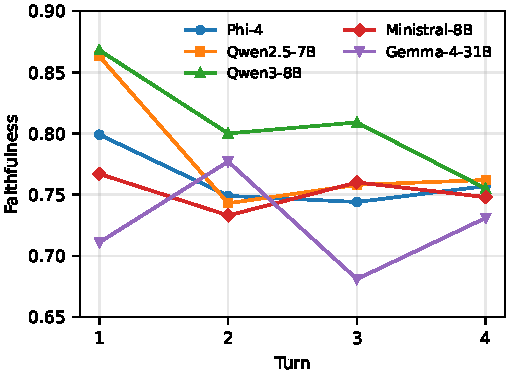
\includegraphics[width=\columnwidth]{fig_generation_turns.pdf}
\caption{Fidelidade da geração por turno para os cinco modelos de linguagem
pequenos (100 conversas). Os modelos mais fiéis declinam significativamente e
convergem para o pelotão, enquanto a recuperação cai de forma bem mais
acentuada (Fig.~\ref{fig:retrieval}).}
\label{fig:generation}
\end{figure}

% ============================================================
\section{Discussão e Limitações}
\label{sec:discussion}
\textbf{O que o benchmark mede.} O Ulysses-MTRAG quantifica uma propriedade da
construção sintética de benchmarks multi-turno: as continuações são
majoritariamente autossuficientes ($11.3\%$ não autossuficientes, por
desenho), de modo que a recuperação ciente do histórico não consegue mostrar
seu valor---nossa análise estratificada confirma que o histórico ajuda apenas
em turnos de esclarecimento e temporais. Apresentamos isso como um achado
diagnóstico sobre pipelines sintéticos multi-turno em um domínio jurídico de
poucos recursos. Benchmarks que pretendam estressar o contexto conversacional
devem impor uma cota maior de turnos não autossuficientes na geração;
deixamos três extensões como trabalho futuro: (a) esse esquema de geração com
cota maior, (b) a elicitação de turnos não respondíveis ($99.3\%$ dos nossos
são respondíveis), que o MTRAG \cite{Katsis2025MTRAG} usa para testar a
abstenção, e (c) uma anotação humana dedicada do pool completo recuperado
para estreitar o limite de confiabilidade do juiz da RQ2.

\textbf{Ameaças à validade.}
\begin{itemize}
  \item[(i)] Avaliamos dois recuperadores (denso e lexical) e encontramos que
  o ranking de estratégias se inverte entre eles; a recuperação híbrida e
  outros codificadores densos podem se comportar de forma diferente novamente,
  então os rankings específicos não devem ser generalizados além das duas
  famílias testadas.
  \item[(ii)] O gerador de continuações, o oráculo e dois modelos avaliados
  são aparentados (mesmo modelo ou família). Mitigamos isso apoiando as
  afirmações principais no eixo de fidelidade sem referência, julgado por um
  modelo de outra família, e observando que um modelo de fora da família
  lidera as métricas baseadas em referência.
  \item[(iii)] A comparação entre famílias tem um modelo por ponto de
  tamanho, então família e tamanho estão parcialmente confundidos.
  Adicionamos uma escada intra-família Qwen (7B/8B/72B) para isolar a escala,
  mas a âncora de 72B também é a autora das perguntas, uma vantagem que não
  conseguimos remover por completo.
  \item[(iv)] Escores baseados em juiz variam entre rodadas de julgamento
  ($\approx0.05$ em valor absoluto, embora o ranking seja estável) e são
  julgados por LLM sobre um pool de recuperação; valores absolutos devem,
  portanto, ser lidos como rankings comparativos, com a confiabilidade
  delimitada na RQ2.
  \item[(v)] O benchmark cobre um corpus legislativo, sessões de quatro
  turnos e continuações sintéticas; diálogo jurídico escrito por humanos pode
  se comportar de forma diferente \cite{Qu2020ORConvQA}.
\end{itemize}

% ============================================================
\section{Conclusão}
Apresentamos o Ulysses-MTRAG, um benchmark sintético multi-turno de RAG
ancorado em humanos para o diálogo legislativo brasileiro. A recuperação
degrada significativamente com a profundidade do diálogo, e a melhor forma de
usar o histórico do diálogo mostrou-se dependente do recuperador: inerte para
a recuperação densa, mas um ganho significativo para o BM25 lexical. A
fidelidade da geração é governada mais pela família do modelo do que pela
escala---um modelo de 8B bem escolhido é competitivo com um modelo de 72B nove
vezes maior---e a degradação da recuperação se propaga para as respostas
geradas apenas fracamente. Por fim, o juiz LLM de relevância concorda com os
rótulos de especialistas em $94\%$ dos documentos que os especialistas
avaliaram explicitamente, com a discordância no pool completo dominada pela
incompletude dos rótulos, e não por erro do juiz. O benchmark, os prompts e o
código serão disponibilizados; um repositório anonimizado acompanha a revisão.

\bibliographystyle{IEEEtran}
\bibliography{references_ictai}

\end{document}
